\documentclass[12pt]{book}
\usepackage{lecturenotes}

\title{{\whitneylightprop \subject{CSci}{30}/\subject{CS}{110} Lecture Notes}\\%
\large{Data Structures and Algorithms}\\
\large{First Semester, \textsc{s.y.} 2019--2020}}
\author{\href{http://penoy.admu.edu.ph/~guadalupe154884/}{Brian Guadalupe}}
% \date{\vfill Last updated: \today}
\date{}

\begin{document}
\pagenumbering{roman}
\maketitle
\newpage
\thispagestyle{empty}
\CatchFileDef{\headfull}{.git/HEAD}{}
\StrGobbleRight{\headfull}{1}[\head]
\StrBehind[2]{\head}{/}[\branch]
\CatchFileDef{\commit}{.git/refs/heads/\branch}{}

\vspace*{\fill}
\begin{center}
\begin{minipage}{0.5\textwidth}
\begin{center}
\small
\textonehalf th edition

Last updated: \today

\vspace{0.5cm}
This revision: \href{https://github.com/alltootechnical/csci30notes/commit/\commit}{\texttt{\commit}} on branch \href{https://github.com/alltootechnical/csci30notes/tree/\branch}{\texttt{\branch}}.
\vspace{1cm}

\copyright{} Copyright 2019 \href{http://penoy.admu.edu.ph/~guadalupe154884/}{Brian Guadalupe}

\vspace{0.5cm}
\ccbysa

This work is licensed under a Creative Commons Attribution-ShareAlike 4.0 International License (\href{http://creativecommons.org/licenses/by-sa/4.0/}{\textsc{cc by-sa 4.0}}).

\vspace{1cm}
Please report errors via GitHub at \href{https://github.com/alltootechnical/csci30notes/issues}{\texttt{github.com/alltootechnical/csci30notes}} or via email at \href{mailto:brian.guadalupe+csci30notes@obf.ateneo.edu}{\texttt{brian.guadalupe@obf.ateneo.edu}}.

\vspace{0.5cm}
\textit{Caveat lector:} This is very much a work in progress; please tread lightly.

\end{center}
\end{minipage}
\end{center}

\newpage
\setcounter{tocdepth}{1}
\tableofcontents
\chapter{Introduction}

What is this course all about? In this chapter, we will answer all of these questions.

\section{Algorithms}
Algorithms are recipes. Just like recipes, algorithms consist of a series of step-by-step instructions or procedures.

\section{Data structures}
Data structures are containers.

\section{Design and implementation goals}

\section{Pseudocode}

\subsection{Pseudocode conventions}


\pagenumbering{arabic}
\part{The Basics}
\chapter{Correctness}
\label{chap:correctness}

One of the two fundamental issues in designing algorithms is \textit{correctness}. In this chapter, we will explore techniques to show and prove the correctness of algorithms.

\section{Defining correctness}
Your notion of correctness might be based on your experience writing code in your introductory CS classes, where you think that your code is correct as long as it matches with the sample output given, or as long as your program does not crash or go to an infinite loop.

However for this course, we would like to make a distinction between empirical correctness and provable correctness.

Simply put, we say that an algorithm is \textit{empirically correct} if it produces the correct output for every input that you only tested or practically use. More often than not, your set of inputs is just a proper subset of all the possible inputs, which is not exhaustive enough if you want to assert the correctness of the algorithm. Since you do not tend to use inputs involving edge cases, you will never know how the algorithm behaves when given unexpected inputs.

On the other hand, we say that an algorithm is \textit{provably correct} if it produces the correct output for every possible input. This does not mean you have exhaustively tested the algorithm for each and every possible input, because that is simply impractical to do. Instead, it means that you have a proof that the algorithm returns the correct output for every input.

We can have the following definition of algorithmic correctness:
\begin{definition}{(\cite{cormen_introduction_2009})}
An algorithm is said to be correct if, for every input instance, it halts with the correct output.
\end{definition}

Why should we care whether or not an algorithm is provably correct? From our experience, we design algorithms such that we know they work given reasonable inputs. But the end-users of these algorithms may not give reasonable inputs all the time.

\begin{example}[A crappy analogy, literally, sort of...]
Consider a chocolate fountain. It takes in melted chocolate as input. The manufacturer guarantees that the chocolate fountain will operate and work properly as intended, provided that it only uses melted chocolate.

\begin{figure}[H]
    \centering
    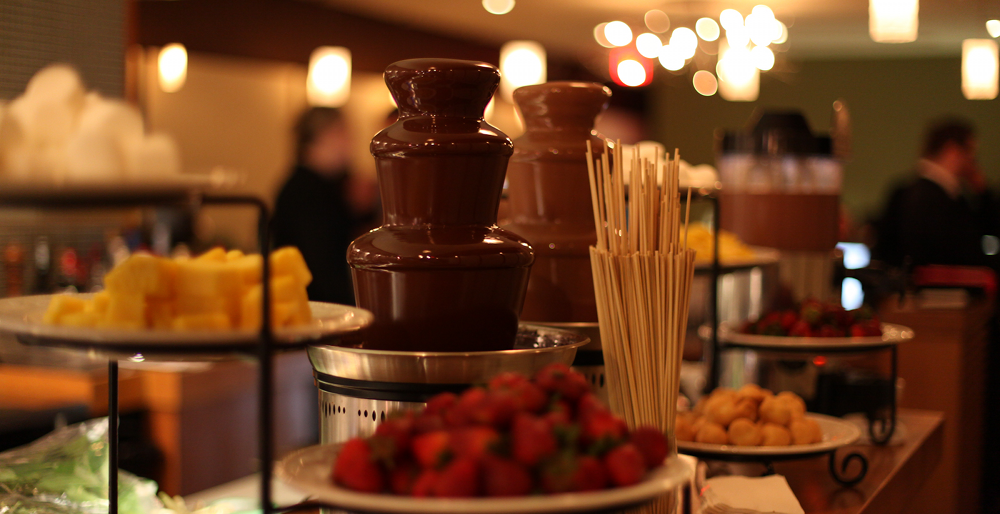
\includegraphics[width=12cm]{figures/Chocolate-Fountains.png}
    \caption{When set up properly, a chocolate fountain can be a perfect party piece}
    % \label{fig:my_label}
\end{figure}

What if the end-user somehow screwed up while operating the chocolate fountain, and a small amount of water made its way through the melted chocolate? Well, it suddenly looks unappetizing... Ew.

\begin{figure}[H]
    \centering
    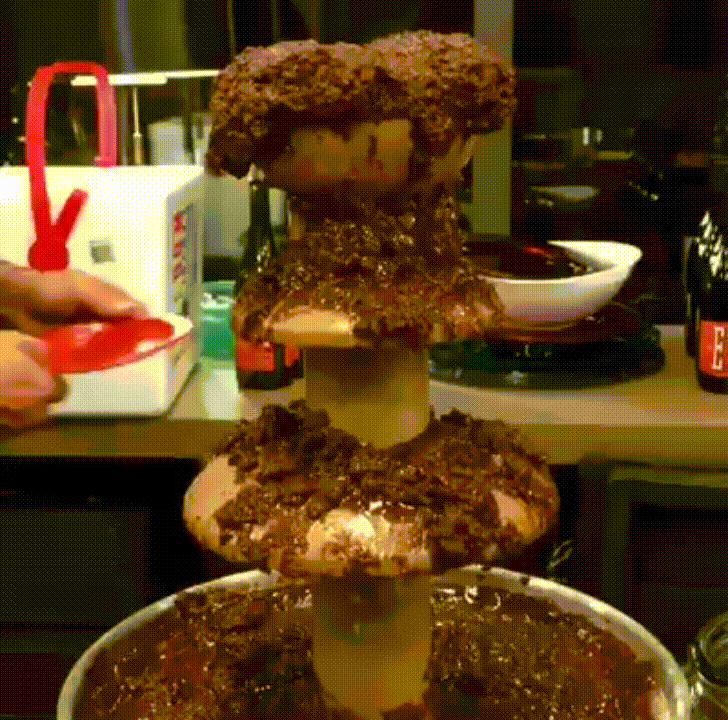
\includegraphics[width=8cm]{figures/fountain_fail.png}
    \caption{Instant disaster, just add water! (View the GIF here: \url{https://i.imgur.com/OX7Gg3R.gifv})}
    % \label{fig:my_label}
\end{figure}

It turns out water and melted chocolate don't mix. What basically happened is that the melted chocolate has seized, meaning the chocolate has clumped together to form chunks. As a result, the chocolate fountain cannot efficiently pump out the chocolate as smoothly like it did previously.

In this case, the end-user cannot complain to the manufacturer that the chocolate fountain is defective, just because it cannot pump the seized chocolate. 
\end{example}

When designing algorithms, we want to ensure that every possible inputs are all accounted for, even edge cases, and in the event that the algorithm gets an unexpected input, it should have been dealt with accordingly. We do not want an algorithm to behave unexpectedly or inconsistently when given unexpected input.

By ensuring that an algorithm is provably correct, we avoid unexpected or undefined behavior. Thus, we ensure that an algorithm \textit{expectedly} returns the correct output.

\section{Mathematical induction}
One technique to prove the correctness of an algorithm is through a proof by induction. This is commonly used when an algorithm only involves a closed-form expression.

Recall that there is a neat formula to get the sum of integers from $1$ to $n$, which is as follows:
\[
\sum_{i=1}^{n} i = \frac{n\left(n+1\right)}{2}
\]

How are we sure that this formula gives the correct answer for all positive integers $n$? We can do a proof by induction by following these steps:
\begin{enumerate}
    \item Base case: Show that the statement is true for the simplest...
    \item Inductive hypothesis: Assume that the statement is true for some $k$.
    \item Inductive step: Show that the statement is true for $k+1$, which uses the inductive hypothesis.
\end{enumerate}

\begin{claim}
The above formula gives the correct answer for integers $n>0$.
\end{claim}
\begin{proof}
    When $n=1$, the sum of integers from $1$ to $1$ is just $1$, and substituting $n$ with $1$ in the formula, we get $\frac{1\left(1+1\right)}{2} = \frac{1\cdot 2}{2} = 1$. Thus the formula is correct for $n=1$.

    Assume that the sum of integers from $1$ to $k$ is $\frac{k\left(k+1\right)}{2}$, for some integer $k < n$. We now show that the formula also holds for $n = k+1$.

    For the inductive step, we want to show that
\[
    \sum_{i=1}^{k+1} i = \frac{\left(k+1\right) \left(k+2\right)}{2}
\]
holds. Then
    \begin{align*}
        \sum_{i=1}^{k+1} i &= 1 + 2 + \cdots + k + \left(k+1\right) \\
        &= \sum_{i=1}^{k} i + \left(k+1\right) \\
        &= \frac{k\left(k+1\right)}{2} + \left(k+1\right) & \text{(by the inductive hypothesis)} \\
        &= \frac{\left(k^2 + k\right) + \left(2k + 2\right)}{2} \\
        &= \frac{k^2 + 3k + 2}{2} \\
        &= \frac{\left(k+1\right) \left(k+2\right)}{2}
    \end{align*}
\end{proof}

\section{Loop invariants}
How do loops work anyway? Recall that a loop consists of a condition, and a series of statements. These statements are always executed, so long as the loop condition holds true. Once the loop condition does not hold anymore, the loop terminates without executing the statements.

If for each iteration, everything inside the loop gets executed, then there must be some condition that holds true at the start of every iteration. Furthermore, the statements inside the loop must make sure that this condition will still hold at the start of the next iteration. This condition is what we call a \textit{loop invariant}. We use loop invariants to prove the correctness of iterative algorithms.

\begin{definition}
A loop invariant is a statement that remains true before, during, and after every iteration of the loop. It satisfies these properties:
\begin{enumerate}
    \item Initialization: A loop invariant is true at the start of the loop.
    \item Maintenance: If a loop invariant is true before the $i$th iteration, it should also remain true before the $\left(i+1\right)$th iteration.
    \item Termination: A loop invariant remains true after the loop ends, which helps us show that the algorithm is correct.
\end{enumerate}
\end{definition}

How do we find a loop invariant? One way is to consider what happens in each iteration of the loop. Try looking at how the value of the variables change throughout an iteration.

\begin{example}
    example box
\end{example}

Another way is to consider what output we should expect the algorithm to return. Most likely, the variable whose value will be returned at the end of the loop is being changed at every iteration.

\begin{example}
    Suppose we have an algorithm for getting the product of integers from $1$ to $n$.
    \begin{algorithm}[H]
        \caption{Get the product of integers from $1$ to $n$ }
        \begin{algorithmic}[1]
            \Require An integer $n$, where $n>0$ 
            \Ensure The product of integers from $1$ to $n$ 
            \Function{IntProd}{$n$}
            \State $P \gets 1$
            \For{$i \gets 1$ to  $n$ }
            \State $P \gets P \cdot i$ 
            \EndFor
            \Return $P$
            \EndFunction
        \end{algorithmic}
    \end{algorithm}

    Notice that inside the for loop, the value of $P$ is updated. For each iteration, what does the value of $P$ represent? 
\end{example}

We can also consider how the algorithm ``builds up'' the answer. This is somewhat related to the previous method of considering what the algorithm is expected to output. Try looking at how it builds up a partial solution at every iteration, so at the end of the loop the answer would now correspond for the entire solution.

\begin{handwritten}
    this is handwritten!
\end{handwritten}

\begin{exercises}

[to-do]
\end{exercises}

\chapter{Efficiency}
\label{chap:efficiency}

In the latter part of your \subject{CSci}{20} class,\footnote{For the remaining students under the old curriculum, \subject{CSci}{20} (called \textit{Introduction to Computing}) is a new course for freshmen. It is pretty much like the CS counterpart of \subject{MIS}{101}.} you talked about the essence of what computing is all about, i.e., what does it exactly mean that a problem is \textit{computable}. More often than not, these problems are considered solved when we can construct an abstract machine such as a finite automaton or a Turing machine that can solve them.

However in this course, we would also like to ask ``What does it mean for a solution to a problem (or a program) to be \textit{efficient}?'' 

In this chapter, we will explore methods to determine the efficiency of an algorithm, as well as establish notations to more conveniently describe efficiency.

\section{Towards defining efficiency}
What does it mean for an algorithm to be efficient? We all have this general idea of efficiency that an algorithm should not use any more of the computer's resources than necessary. 

Since the real world we live in is finite and limited, we cannot afford to use solutions that unnecessarily expend a lot of resources. So there is a need to efficiently allocate resources so that more of those can be used in the future. 

In the field of computing, our main resources are \textit{time} and \textit{space}. More specifically, time refers to how long an algorithm takes to run, while space refers to how much memory an algorithm consumes.

Let us formalize our notion of what an efficient algorithm is by proposing the following definition.
\begin{claim}[Proposed definition \#1, from \cite{kleinberg_algorithm_2006}]
An algorithm is efficient if, when implemented, it runs quickly on real input instances.
\end{claim}

But wait, what do we mean by ``quickly'' here?

% It is not enough that a program is \textit{provably correct}, but also it must be \textit{provably efficient}.

\section{Measuring efficiency}
\label{sec:measuring-efficiency}

How do we measure efficiency? In real life, engineers often use \textit{benchmarks} to ensure that their work conforms to a standard. They repeatedly take measurements of different properties while manipulating or tweaking some of the variables and observe the outcomes. 

Recall that a program takes in some input and gives out some output, but the way time and memory are consumed are very much dependent on how the program deals or what the program does on the given input. So we usually measure efficiency in terms of time and memory consumption.

More concretely, we can measure the execution time of a program using built-in methods such as \texttt{System.currentTimeMillis()} in Java and \texttt{timeit.timeit()} in Python.

\begin{example}[Benchmarking]
\label{ex:running_time}

% [TO-DO: Rewrite this example!]

Here we have two functions that both compute the sum of integers from $1$ to $n$.

% \begin{listing}[H]
% \begin{minted}{python}
% def int_sum(n):
%     S = 0
%     for i in range(1, n+1):
%         S += i
%     return S
% \end{minted}
% \caption{Get the sum of all integers from $1$ to $n$}
% \label{lst:int_sum}
% \end{listing}
\begin{minipage}{0.45\textwidth}
\begin{listing}[H]
\begin{minted}{python}
def intsum(n):
    S = 0
    for i in range(1, n+1):
        S = S + i
    return S
\end{minted}
\label{lst:intsum}
\end{listing}
\end{minipage}\hfill
\begin{minipage}{0.45\textwidth}
\begin{listing}[H]
\begin{minted}{python}
def intsum2(n):
    return n*(n+1)//2
\end{minted}
\label{lst:intsum2}
\end{listing}
\end{minipage}

Try running both \texttt{intsum} and \texttt{intsum2} with succeeding powers of $10$, starting from $1$, $10$, $100$, $1000$, and so on. What do you notice? Does the program take a little bit longer for large values of $n$?

If we record the actual running time of the program for each power of $10$, we get the following plot shown in Figure~\ref{fig:intsum_runtime}.

\begin{figure}[H]
	\centering
	\begin{tikzpicture}
		\begin{loglogaxis}[
		    width=0.8\textwidth,
		    height=8cm,
			xmin=1, xmax=1e9,
			ymin=1e-6, ymax=100,
			xlabel={$n$}, 
			ylabel={Running time (seconds)},
			grid=major,
			legend pos=north west,
			legend cell align=left,
			tick scale binop=\times
		]
		\addplot[thick, attblue, mark=*] table[x=n, y=intsum] {plots/intsum.txt};
		\addplot[thick, attred, mark=*] table[x=n, y=intsum2] {plots/intsum.txt};
		\legend{\texttt{intsum},\texttt{intsum2}}
		\end{loglogaxis}
	\end{tikzpicture}%
	\label{fig:intsum_runtime}
\end{figure}

% \begin{figure}[H]
% 	\centering
% 	\begin{tikzpicture}
% 		\begin{loglogaxis}[
% 		    width=0.8\textwidth,
% 			xmin=1, xmax=1e9,
% 			ymin=1e-6, ymax=100,
% 			xlabel={$n$}, ylabel={Running time (sec)},
% 			grid=major,
% 			legend pos=south east,
% 			legend cell align=left,
% 			tick scale binop=\times
% 		]
% 		\addplot[thick, attblue, only marks] table[x=n, y=time] {plots/intsum_runtime.txt};
% 		\addplot[thick, attblue] table[x=n, y=time] {plots/intsum_runtime.txt};
% 		\end{loglogaxis}
% 	\end{tikzpicture}%
% 	\caption{Running time of \texttt{int\_sum}}
% 	\label{fig:int_sum_runtime}
% \end{figure}

% Note that the points are plotted with a log-log scale, so if it seems that they follow a linear trend, it is actually an \textit{exponential} trend. As the input $n$ increases by a tenfold, the running time will also increase by a tenfold. Running \texttt{int\_sum(10000000)} takes around half a second, while \texttt{int\_sum(100000000)} takes about $5$ seconds, and \texttt{int\_sum(1000000000)} takes about $50$ seconds to run.
\end{example}

The problem with benchmarking when it comes to computer programs is that not all computers are created equally; the specifications and parts within it wildly differ from one computer to another. Some programs might run quickly on one computer, but very slowly in another. You need to have the same machine setup every time you compare algorithms. In other words, \textbf{efficiency is relative to physical constraints.}

% ripped off from ASPC-B 2018 slides
Another problem is that we have to implement code first, and for many people this is a waste of time. When you write code, chances are you simply end up tweaking the code, thus you would not gain any insight on why the program is slow, or even how to design faster programs in the first place. 

% ripped off from ASPC-B 2018 slides
You may be thinking, ``My program is really not that slow, you just need a faster computer!'' But how do we build faster computers? ``You just need to buy faster parts!'' But how do we build faster parts? ``You just need to get faster materials!'' But how do we get faster materials? ``You just need... \textit{to get a faster universe!}''

\section{Model of computation}
Instead of looking at the actual running time of each of the operations, let us assume that the operations have a fixed cost at some level. Which operations we consider available and their respective costs form a particular \textit{model of computation}. 

Now, efficiency is dependent on the algorithm that the program uses, that is, it is now dependent on how the higher-level operations are implemented with lower-level operations.

We can measure program efficiency like this:
\begin{enumerate}
    \item Choose a set of operations that we consider to have a fixed cost.
    \item Measure the average cost for each of those operations.
    \item Count number of operations we perform for each type of operation.
    \item Then the total cost would be the sum of the number of operations times the cost of the operation, over all operations.
\end{enumerate}

But we can do better! We could actually do away with measuring in terms of seconds or bytes, since the actual numbers would be heavily dependent on the hardware. Instead, we choose a set of operations such that they would have the same average cost. Then the total cost would simply be equal to the total number of operations.

For this course, we will be using what is called the \textit{random-access machine} model of computation, or the RAM model for short.
\begin{definition}
The random-access machine (RAM) model of computation assumes that the following primitive operations have a cost of $1$:
\begin{enumerate}
    \item assigning a value to a variable,
    \item fetching the value of a variable,
    \item calling a method or function,
    \item performing an arithmetic operation,
    \item comparing two values,
    \item indexing into an array,
    \item following an object reference, and
    \item returning from a method.
\end{enumerate}
\end{definition}

\begin{example}[Counting operations]
\label{ex:countingops}

We consider \texttt{int\_sum} as shown in Listing~\ref{lst:int_sum}, but we rewrite it first using pseudocode.
\begin{algorithm}[H]
    \label{alg:intsum}
    \caption{Calculate the sum of all integers from $1$ to $n$}
    \begin{algorithmic}[1]
        \Require An integer $n$
        \Ensure The sum $S$ of all integers from $1$ to $n$
        \Function{IntSum}{$n$}
            \State $S \gets 0$
            \For{$i \gets 1$ to $n$}
            \State $S \gets S+i$
            \EndFor
            \Return $S$
        \EndFunction
    \end{algorithmic}
\end{algorithm}

Before we can start counting the number of operations, we need to establish what model of computation to use. In our case, we will use the RAM model as defined earlier.

To make things easier, we will rewrite the for loop in \textsc{IntSum} using a while loop as shown in Algorithm~\ref{alg:intsumwhile}. It is not hard to see that both are equivalent.

\begin{algorithm}[H]
    \label{alg:intsumwhile}
    \caption{Calculate the sum of all integers from $1$ to $n$}
    \begin{algorithmic}[1]
        \Require An integer $n$
        \Ensure The sum $S$ of all integers from $1$ to $n$
        \Function{IntSum}{$n$}
            \State $S \gets 0$
            \State $i \gets 1$
            \While{$i \le n$}
            \State $S \gets S+i$
            \State $i \gets i+1$
            \EndWhile
            \Return $S$
        \EndFunction
    \end{algorithmic}
\end{algorithm}

We can already see $2$ assignment operations that initialize the values of $S$ and $i$. There are also $2$ assignment operations inside the while loop, which updates the value of $S$ and increments the value of $i$. Since the loop goes through $n$ iterations, there are $2n$ assignments in total. Overall, \textsc{IntSum} has $2n+2$ assignment operations.

In the loop, we fetch the values of $i$ and $n$, as well as the values of $S$ and $i$ to update $S$, and $i$ again to increment its value. Then we have $5$ variable fetch operations, but those are happening within the loop, so we have $5n$ variable fetch operations in total. But before we exit the loop, we check the condition one last time, which involves fetching the values of $i$ and $n$. Overall, \textsc{IntSum} has $5n+2$ variable fetch operations.

Additionally (pun intended), there are $2$ addition operations in the loop, one for adding $i$ to $S$ and another one for incrementing $i$, i.e. adding $1$ to $i$. These are done per iteration, so there are $2n$ addition operations overall.

For each iteration of the loop, a single comparison operation is done for comparing the values of $i$ and $n$, for a total of $n$ comparison operations. Before exiting the loop, we check the condition one last time, which also involves a comparison. Thus \textsc{IntSum} has $n+1$ comparison operations.

To get the total number of operations in \textsc{IntSum}, we simply get the sum per operation, so \textsc{IntSum} has $T\left(n\right) = \left(2n+2\right) + \left(5n+2\right) + 2n + \left(n+1\right) + 1 = \boxed{10n+6}$ operations all in all.
\end{example}

In the preceding example, we have shown that the \textit{running time} of \textsc{IntSum} is $T\left(n\right) = 10n+6$. Notice that the number of operations grows as the input gets larger, that is why it is a function of the input size.

So here's the takeaway: \textbf{efficiency only matters when the input size is large.} As the size of the input gets larger, the lower-order terms will be overshadowed by the highest-order term.

\section{Orders of growth}

In the previous section, we have seen how the size of the input affects the running time of an algorithm. But it is also possible that the running time changes even when two different inputs of the same size are given.

\begin{example}[Searching in a list]
\label{ex:searching-list}
We have the following algorithm to find an element in some list. If such an element is found, it will return its (one-based) position in the list. Otherwise, it returns $0$.

\begin{algorithm}[H]
    \label{alg:search-element}
    \caption{Get the index of an element $e$ in a list $L$, if it exists}
    \begin{algorithmic}[1]
        \Function{SearchElement}{$L$, $e$}
            \For{$i \gets 1$ to $\left|L\right|$}
            \Comment{$\left|L\right|$ is the length of the list $L$}
                \If{$L_i = e$}
                    \Return $i$
                \EndIf
            \EndFor
            \Return $0$
            \Comment{if $e$ is not found in $L$}
        \EndFunction
    \end{algorithmic}
\end{algorithm}

Suppose we want to search in the list $\List{50,84,1,96,5}$. For which inputs can we achieve the minimum running time? In other words, which values of $e$ can we give so that \textsc{Search-Element} runs with the fewest number of operations?

Since the for loop checks the list from the first element to the last element, if the first element is equal to $e$, then the algorithm returns $1$ and terminates. We did not need to deal with the remaining elements! So we consider this as the algorithm's \textit{best case}.

Now let's determine the best case running time of \textsc{Search-Element}. We are still going to use the same model of computation that we have in Example~\ref{ex:countingops}.

What would happen if $e$ is not in the list?

\end{example}

Do we \textit{really} need to know the exact number of operations? Even minor changes to the implementation of an algorithm can change its running time.

However, if we were to analyze larger and more complicated programs for efficiency, counting the number of operations can get very difficult very quickly. In some cases, it may not even be possible at all to determine the exact running time of a program, and so it will not be worth the effort.

Maybe we only care about how \textit{fast} the running time grows. Instead of saying that ``the running time of \textsc{IntSum} is $10n+6$,'' it's enough to say that ``the running time of \textsc{IntSum} grows proportionally to $n$.'' Our goal, then, is to simplify algorithm analysis by getting rid of irrelevant information. How?

\section{Asymptotic analysis}
\label{sec:asymptotic}

When we are dealing with input sizes that are large enough so that only the rate of growth of the running time matters, we are looking at the \textit{asymptotic} efficiency of an algorithm. Why call it ``asymptotic?'' If you recall your lesson about conic sections in your precalculus class, you have encountered the concept of an asymptote, which comes from the Greek word meaning ``not falling together.'' 

Just like how a curve \textit{almost} approaches an asymptote but never touches it, we say that two functions are \textit{asymptotically equal} if they \textit{almost} approach one another but never intersect at a later point.\footnote{Formally speaking, we say that two functions $f$ and $g$ are asymptotically equal (sometimes denoted as $f \sim g$) if and only if $\lim_{x \to \infty}{\frac{f\left(x\right)}{g\left(x\right)}}$ exists and is equal to $1$. But you don't need to know this fact for this course.} We can see this in action in the following example.

\begin{example}[Comparing growth of functions]
% \url{https://www.desmos.com/calculator/k4p7sewkq2}

Suppose we have some algorithm that has a running time of $T\left(n\right) = n^2 + 3n + 2$. We want to compare how it grows as input size $n$ gets larger along with other functions like $f\left(n\right) = n^2$, $g\left(n\right) = n$, and $h\left(n\right) = 2^n$ by sketching their plots, as shown in Figure~\ref{fig:growth_comp}. \footnote{An interactive version of the plots is also available at \url{https://www.desmos.com/calculator/k4p7sewkq2}.}

\begin{figure}[H]
	\centering
	\begin{tikzpicture}
		\begin{axis}[
		    width=0.8\textwidth,
			xmin=0, xmax=4,
			ymin=0, ymax=6,
			xlabel={$n$}, ylabel={Running time},
			grid=major,
			legend pos=south east,
			legend cell align=left
		]
		\addplot[ultra thick, attblue, samples=100]  {x^2 + 3*x + 2};
		\addplot[thick, attyellow, samples=100]  {x^2};
		\addplot[thick, attred, samples=100]  {x};
		\addplot[thick, attgreen, samples=100]  {2^x};
		\legend{$T\left(n\right)$, $f\left(n\right)$, $g\left(n\right)$, $h\left(n\right)$}
		\end{axis}
	\end{tikzpicture}%
	\caption{Growth of $T\left(n\right)$ compared to $f\left(n\right)$, $g\left(n\right)$, and $h\left(n\right)$}
	\label{fig:growth_comp}
\end{figure}

As expected, the four plots all look different. But if we zoom out further as in Figure~\ref{fig:growth_comp_zoomout}, we get the following.

\begin{figure}[H]
	\centering
	\begin{tikzpicture}
		\begin{axis}[
		    width=0.8\textwidth,
			xmin=0, xmax=20,
			ymin=0, ymax=200,
			xlabel={$n$}, ylabel={Running time},
			grid=major,
			legend pos=south east,
			legend cell align=left
		]
		\addplot[ultra thick, attblue, samples=100, domain=0:20]  {x^2 + 3*x + 2};
		\addplot[thick, attyellow, samples=100, domain=0:20]  {x^2};
		\addplot[thick, attred, samples=100, domain=0:20]  {x};
		\addplot[thick, attgreen, samples=100, domain=0:8]  {2^x};
		\legend{$T\left(n\right)$, $f\left(n\right)$, $g\left(n\right)$, $h\left(n\right)$}
		\end{axis}
	\end{tikzpicture}%
	\caption{Growth of $T\left(n\right)$ compared to $f\left(n\right)$, $g\left(n\right)$, and $h\left(n\right)$}
	\label{fig:growth_comp_zoomout}
\end{figure}

As before, the plot of $T\left(n\right)$ still looks different from both $g\left(n\right)$ and $h\left(n\right)$, but notice that both $T\left(n\right)$ and $f\left(n\right)$ look the same, as if they are almost approaching (or closely following) one another.

\end{example}


\subsection{$\Theta$-notation}
\begin{definition}[\cite{cormen_introduction_2009}]
For a given function $g \left(n\right)$, we denote by $\bigTheta{g \left(n\right)}$ the set of functions
\[
\bigTheta{g \left(n\right)} = \left\{f\left(n\right) \mid \exists c_1, c_2, n_0 > 0 \text{ such that } 0 \le c_1 \cdot g \left(n\right) \le f \left(n\right) \le c_2 \cdot g \left(n\right) \text{ for all } n \ge n_0 \right\}.
\]
\end{definition}

\subsection{$O$-notation}
\begin{definition}[\cite{cormen_introduction_2009}]
For a given function $g \left(n\right)$, we denote by $\bigO{g \left(n\right)}$ (pronounced ``big-oh of $g$ of $n$'' or sometimes just ``oh of $g$ of $n$'') the set of functions
\[
\bigO{g \left(n\right)} = \left\{f\left(n\right) \mid \exists c, n_0 > 0 \text{ such that } 0 \le f \left(n\right) \le c \cdot g \left(n\right) \text{ for all } n \ge n_0 \right\}.
\]
\end{definition}

\subsection{$\Omega$-notation}
\begin{definition}[\cite{cormen_introduction_2009}]
For a given function $g \left(n\right)$, we denote by $\bigOmega{g \left(n\right)}$ (pronounced ``big-omega of $g$ of $n$'' or sometimes just ``omega of $g$ of $n$'') the set of functions
\[
\bigOmega{g \left(n\right)} = \left\{f\left(n\right) \mid \exists c, n_0 > 0 \text{ such that } 0 \le c \cdot g \left(n\right) \le f \left(n\right) \text{ for all } n \ge n_0 \right\}.
\]
\end{definition}

\begin{theorem}[\cite{cormen_introduction_2009}]
\label{thm:bigtheta}
For any two functions $f\left(n\right)$ and $g\left(n\right)$, we have $f\left(n\right) = \bigTheta{g \left(n\right)}$ if and only if $f\left(n\right) = \bigO{g \left(n\right)}$ and $f\left(n\right) = \bigOmega{g \left(n\right)}$.
\end{theorem}

\begin{exercises}
\begin{enumerate}
    \item The following algorithm counts the number of multiples of $1, 2, 3, \ldots, n$ from an array $A$ of $n$ integers (indexed $1$ to $n$), and stores and returns the counts in a separate array.
    \begin{algorithm}[H]
        \caption{Count the number of multiples of $1, 2, 3, \ldots, n$ given an array}
        \begin{algorithmic}[1]
            \Function{CountMultiples}{$A$}
            \For{$m \gets 1$ to $n$}
                \State $\mathrm{count}[m] \gets 0$
            \EndFor
            % \State $\mathrm{count}_1 \gets n$
            % \Comment{all numbers are divisible by $1$}
            \For{$i \gets 1$ to $n$}
                \For{$m \gets 1$ to $n$}
                    \If{$A[i] \bmod{m} = 0$}
                        \State $\mathrm{count}[m] \gets \mathrm{count}[m] + 1$
                    \EndIf
                \EndFor
            \EndFor
            \Return $\mathrm{count}$
            \EndFunction
        \end{algorithmic}
    \end{algorithm}
    \begin{enumerate}
        \item Suppose our input array is $\List{10,17,8,240,15}$. \textbf{Exactly} how many operations are carried out? Determine the number of operations attributable for each line, then get the total at the end.
        \item For an array of length $n$ (assume worst-case), how many operations are carried out? Determine the number of operations attributable for each line, then get the total at the end. Provide your answers in terms of $n$.
        \item Express the worst-case running time (i.e., total number of operations) using big-$O$ notation.
        
    \end{enumerate}
    
    \item Prove or disprove each of the following:
    \begin{enumerate}
        \item $3^n + 100n^2 + n^{200}$ is $\bigO{2^n}$
        \item $2\sqrt{n} + 34$ is $\bigO{n^2}$
        \item $6n \log{n} + 4n$ is $\bigO{n}$
        \item $n^3 + n^2 \log{n} + n \sqrt{n}$ is $\bigO{n^3}$
        \item $4^{n-1}$ is $\bigO{3^{n+1}}$
    \end{enumerate}
    
    \item (\cite{graham_concrete_1994}) What's wrong with the following statement? ``Since $n = \bigO{n}$ and $2n = \bigO{n}$ and so on, we have $\sum_{k=1}^n kn = \sum_{k=1}^n \bigO{n} = \bigO{n^2}$.''
    
    \item How much bigger of an input can a program with the following running times process in the same time, given a computer twice as fast?
    
    \noindent
    \begin{enumerate*}
        \item $\bigO{n}$
        \item $\bigO{n^2}$
        \item $\bigO{n^3}$
        \item $\bigO{n^4}$
        \item $\bigO{2^n}$
    \end{enumerate*}

    \item [\challenge] Jose has discovered an elegant way of counting the number of divisors using a modified version of the sieve of Eratosthenes.
    
    \begin{algorithm}[H]
        \caption{Jose's divisor sieve}
        \begin{algorithmic}[1]
            \Function{DivisorSieve}{}
            % \State initialize $\mathrm{divisors}$ as an array of length $n+1$ filled with $0$
            \For{$i \gets 1$ to $n$}
                \State $\mathrm{divisors}[i] \gets 0$
            \EndFor
            \For{$i \gets 1$ to $n$}
                \For{$j \gets i$ to $n$ by $i$}
                    \Comment{for each multiple of $i$ less than or equal to $n$}
                    \State $\mathrm{divisors}[j] \gets \mathrm{divisors}[j] + 1$
                \EndFor
            \EndFor
            \Return{divisors}
            \EndFunction
        \end{algorithmic}
    \end{algorithm}
    
    He says, ``At first glance, it may seem that the time complexity is $\bigO{n^2}$ because of the nested for loop, but actually it runs in just $\bigO{n \log n}$ time!'' Prove or disprove his claim.
    
    \item [\challenge] Prove Theorem~\ref{thm:bigtheta}.
    
\end{enumerate}
\end{exercises}
\chapter{Recursion}
\label{chap:recursion}

Recursion is one of the fundamental concepts in computer science. In this chapter, you will see how recursion differs from iteration, how it manifests in some real-world problems, and some examples of algorithms that use recursion.

If you want to learn more about recursion, you may read Chapter~\ref{chap:recursion}.

\section{What is recursion?}
We know different ways to express repetitive processes. In your first programming class, you have encountered the concept of loops. 

\begin{definition}
An object has a recursive behavior if it satisfies these properties:
\begin{enumerate}
    \item It has a terminating \textit{base case} that does not use recursion.
    \item Whenever it calls itself, the problem gets simplified towards the base case.
\end{enumerate}
\end{definition}

Basically, the main idea behind recursion is that 

\section{Thinking recursively}


\section{Recursive algorithms}

\subsection{Recursive definitions}
Why do we sometimes prefer recursion to iteration? One of the main reasons is that some methods and functions have a straightforward definition that uses recursion. This implies the implementation of these functions will be more elegant than their iterative counterparts.

\begin{example}[Getting the $n$th factorial]
The factorial has the following recursive definition:
\[
n! = \begin{cases}
1 & \text{if } n=0 \\
n\cdot\left(n-1\right)! & \text{otherwise}
\end{cases}
\]

Implementing this would just involve directly copying the definition, so the pseudocode for getting the $n$th factorial is as follows.

\begin{algorithm}[H]
    \caption{A recursive algorithm to get the $n$th factorial}
    \begin{algorithmic}[1]
    \Require An integer $n$, where $n \ge 0$
    \Ensure The value of $n!$
    \Function{Factorial}{$n$}
        \If{$n=0$}
        \Return $1$
        \Else
        \Return $n \cdot \text{\Call{Factorial}{$n-1$}}$
        \EndIf
    \EndFunction
\end{algorithmic}
\end{algorithm}

Suppose we want to compute \Call{Factorial}{$5$}. Then this call will be evaluated by repeatedly applying the recursive definition, as illustrated below. 
\begin{figure}[H]
    \centering
    \begin{align*}
    & \Call{Factorial}{5} \\
    &\implies 5 \cdot \Call{Factorial}{4} \\
    &\implies 5 \cdot \left( 4 \cdot \Call{Factorial}{3} \right) \\
    &\implies 5 \cdot \left( 4 \cdot \left( 3 \cdot \Call{Factorial}{2} \right) \right) \\
    &\implies 5 \cdot \left( 4 \cdot \left( 3 \cdot \left( 2 \cdot \Call{Factorial}{1} \right) \right) \right) \\
    &\implies 5 \cdot \left( 4 \cdot \left( 3 \cdot \left( 2 \cdot \left( 1 \cdot \Call{Factorial}{0} \right) \right) \right) \right) \\
    &\implies 5 \cdot \left( 4 \cdot \left( 3 \cdot \left( 2 \cdot \left( 1 \cdot 1 \right) \right) \right) \right) \\
    &\implies 5 \cdot \left( 4 \cdot \left( 3 \cdot \left( 2 \cdot 1 \right) \right) \right) \\
    &\implies 5 \cdot \left( 4 \cdot \left( 3 \cdot 2 \right) \right) \\
    &\implies 5 \cdot \left( 4 \cdot 6 \right) \\
    &\implies 5 \cdot 24 \\
    &\implies 120
    \end{align*}
    \caption{Trace of the function call for \Call{Factorial}{$5$}}
    % \label{fig:my_label}
\end{figure}

Thus \Call{Factorial}{$5$} returns $120$, as expected.
\end{example}

\subsection{Recursive structures}
Another reason to prefer recursion to iteration is that some problems have a naturally recursive structure.

\begin{example}[Searching for a file within a directory]
How do you search for a file within a directory? You typically would use the search feature that's built-in. Now imagine that this feature did not exist at all. What would you do?



\begin{algorithm}[H]
    \caption{f}
    \begin{algorithmic}[1]
    \Require A directory $\textit{dir}$ and a $\textit{file}$
    \Ensure \algtrue\ if file is found, \algfalse\ otherwise
    \Function{FindFile}{\textit{dir}, \textit{file}}
        \ForEach{file $f \in \text{\Call{ListFiles}{\textit{dir}}}$}
            \If{$f = \mathit{file}$}
            \Return \algtrue
            \EndIf
        \EndFor
        \ForEach{$\textit{subdir} \in \text{\Call{ListDirectories}{\textit{dir}}}$}
            \Return \Call{FindFile}{\textit{subdir}, \textit{file}}
        \EndFor
        \Return \algfalse
    \EndFunction
\end{algorithmic}
\end{algorithm}
\end{example}

\section{Divide-and-conquer}
One of the four algorithmic paradigms\footnote{So far, we have brute force (or complete search), and divide-and-conquer. In later chapters, we will encounter the other two algorithmic paradigms.} we will cover for this course is \textit{divide-and-conquer}. The divide-and-conquer paradigm involves three steps:
\begin{enumerate*}
    \item \textbf{divide} the original problem into several smaller instances of the problem (called \textit{subproblems}),
    \item \textbf{conquer} these subproblems by solving each of them recursively, and then
    \item \textbf{combine} the solutions to the subproblems into an overall solution to the original problem.
\end{enumerate*}

Applications of divide-and-conquer can be seen from many fields. 

One of the prototypical example of a divide-and-conquer algorithm is \textit{merge sort}.

\subsection{Exponentiation}
The exponentiation operation is typically defined as a series of repeated multiplications, where to get the value of $x^n$, you would multiply the base $x$ by itself $n$ number of times.
\[
x^n = \underbrace{x \cdot x \cdot \cdots \cdot x}_{\text{$n$ times}}
\]

From this definition, we can implement a simple iterative algorithm that computes $x^n$.
\begin{algorithm}[H]
    \caption{An iterative algorithm for exponentiation}
    \begin{algorithmic}[1]
    \Require A real number $x$ and an integer $n$, where $n \ge 0$
    \Ensure The value of $x^n$
    \Function{Pow}{$x$, $n$}
    \State $P \gets 1$
    \For{$i \gets 1$ to $n$}
        \State $P \gets P \cdot x$
    \EndFor
    \Return $P$
    \EndFunction
    \end{algorithmic}
\end{algorithm}

It is not hard to see that \textsc{Pow} runs in $\bigO{n}$ time. For example, if we want to compute $x^8$ for some $x$, \Call{Pow}{$x$, $8$} would involve $8$ multiplications.

But we can do better! Instead of considering the exponentiation operation as a series of repeated multiplications, we can also define exponentiation as a series of \textit{repeated squarings}. If we use the fact that
\[
    x^n = x^{n/2} \cdot x^{n/2} = \left(x^{n/2}\right)^2 = \left(x^2\right)^{n/2},
\]
then we can compute $x^8$ in just $3$ multiplications! We can do the following series of operations:
\begin{align*}
    x^8 &= x^4 \cdot x^4 \\
    x^4 &= x^2 \cdot x^2 \\
    x^2 &= x \cdot x
\end{align*}
What if the exponent $n$ is odd? We can use the property
\[
    x^n = x \cdot x^{n-1} = x \cdot \left(x^2\right)^{\frac{\left(n-1\right)}{2}}
\]
since we know that $n-1$ is even when $n$ is odd. Using these two properties, we can now define the exponentiation operation as a series of repeated squarings. We have:
\[
x^n = \begin{cases}
    \left(x^2\right)^{n/2} & \text{if $n$ is even} \\
    x \cdot \left(x^2\right)^{\frac{\left(n-1\right)}{2}} & \text{if $n$ is odd}
\end{cases}
\]

Then the implementation would look like this:
\begin{algorithm}[H]
    \caption{A recursive algorithm for exponentiation by repeated squaring}
    \begin{algorithmic}[1]
    \Require A real number $x$ and an integer $n$, where $n \ge 0$
    \Ensure The value of $x^n$
    \Function{FastPow}{$x$, $n$}
    \If{$n = 0$}
        \Return $1$
    \ElsIf{$n = 1$}
        \Return $x$
    \ElsIf{$n \bmod 2 = 0$}
    \Comment{if $n$ is even}
        \Return \Call{FastPow}{$x \cdot x$, $n/2$}
    \ElsIf{$n \bmod 2 \ne 0$}
    \Comment{if $n$ is odd}
        \Return $x \cdot \text{\Call{FastPow}{$x \cdot x$, $\left(n-1\right)/2$}}$
    \EndIf
    \EndFunction 
    \end{algorithmic}
\end{algorithm}

\subsection{Merge sort}
Merge sort is a sorting algorithm that uses divide-and-conquer. It involves three steps:
\begin{enumerate}
    \item \textbf{Divide:} Split the array of length $n$ into two subarrays, each of length $n/2$.
    \item \textbf{Conquer:} Sort the two subarrays using merge sort.
    \item \textbf{Combine:} Merge the two subarrays together to form the sorted array.
\end{enumerate}

\begin{algorithm}[H]
    \caption{The merging step in merge sort}
    \begin{algorithmic}[1]
        \Require Two sorted arrays $L$ and $R$
        \Ensure A single sorted array $S$
        \Function{Merge}{$L$, $R$}
            \If{$L$ is empty}
                \Return $R$
            \ElsIf{$R$ is empty}
                \Return $L$
            \EndIf
            \If{$\text{\Call{First}{$L$}} \le \text{\Call{First}{$R$}}$}
                \Return \Call{Cons}{\Call{First}{$L$}, \Call{Merge}{\Call{Rest}{$L$}, $R$}}
            \Else
                \Return \Call{Cons}{\Call{First}{$R$}, \Call{Merge}{$L$, \Call{Rest}{$R$}}}
            \EndIf
        \EndFunction
    \end{algorithmic}
\end{algorithm}

\begin{algorithm}[H]
    \caption{The main merge sort algorithm}
    \begin{algorithmic}[1]
        \Require An array $A$
        \Ensure A sorted array $S$
        \Function{MergeSort}{$A$}
            \If{$\text{\Call{Length}{$A$}} = 1$}
            \Return $A$
            \EndIf
            \State split $A$ into two halves $L$ and $R$
            \State $L \gets \text{\Call{MergeSort}{$L$}}$
            \State $R \gets \text{\Call{MergeSort}{$R$}}$
            \State $S \gets \text{\Call{Merge}{$L$, $R$}}$
            \Return $S$
        \EndFunction
    \end{algorithmic}
\end{algorithm}

\begin{example}[Merge sort]
f
\end{example}

\subsection{Analyzing divide-and-conquer algorithms}
We can express the running time of divide-and-conquer algorithms using a \textit{recurrence}.

Let $T\left(n\right)$ be the running time when input size is $n$. When the problem size is small enough (i.e., $n \le c$ for some constant $c$), then we can just use the straightforward solution that takes $\bigO{1}$ time. 

Suppose that upon dividing the problem, it yielded $a$ subproblems, each of which is $1/b$ of the original. Solving one subproblem of size $n/b$ would have a running time of $T\left(n/b\right)$. To solve $a$ subproblems, it would take $a T\left(n/b\right)$ time.

If it took $D\left(n\right)$ time to divide into subproblems, and $C\left(n\right)$ time to combine all solutions into the overall solution, we have the following recurrence:
\[
T\left(n\right) = \begin{cases}
    \bigO{1} & \text{if $n \le c$}\\
    a T\left(n/b\right) + D\left(n\right) + C\left(n\right) & \text{otherwise}
\end{cases}
\]

Later in this chapter, we will see how we can solve some recurrences of this form.

\begin{example}[Running time of merge sort]
To simplify our analysis, assume that the problem size is a power of $2$. Then the divide step would yield two subproblems of exactly size $n/2$.

When the size is exactly $1$, we can just use the straightforward solution that takes $\bigO{1}$ time.

For $n > 1$, we can derive the running time as follows:
\begin{enumerate}
    \item \textbf{Divide:} The divide step splits the array into two equal subarrays. Getting the subarray takes $\bigO{n}$ at the worst case. Thus $D\left(n\right) = \bigO{n}$.
    \item \textbf{Conquer:} We recursively solve two subproblems, each of size $n/2$, which contributes $2T(n/2)$ to the running time.
    \item \textbf{Combine:} The merging step goes through every element of the two subarrays each of size $n/2$, so it takes $\bigO{n}$ time. Thus $C\left(n\right) = \bigO{n}$.
\end{enumerate}

Therefore, the worst-case running time of merge sort has the recurrence
\[
T\left(n\right) = \begin{cases}
    \bigO{1} & \text{if $n = 1$}\\
    2 T\left(n/2\right) + \bigO{n} & \text{otherwise}
\end{cases}
\]

Solving this recurrence, we eventually get $T\left(n\right) = \bigO{n \log n}$. How?
\end{example}

\section{Solving recurrences}

\subsection{Recursion trees}
A recursion tree is a diagram of all the recursive calls made, and the amount of work done in each call. Each node in the recursion tree represents the cost of a single subproblem within a tree of recursive calls.

\subsection{Master theorem}
The master theorem serves as a ``cookbook'' for solving recurrences of the form
\[
T\left(n\right) = aT\left(n/b\right) + f\left(n\right)
\]
where $a \ge 1$ and $b>1$ are constants, and $f\left(n\right)$ is asymptotically positive.

Here, $n/b$ may not be an integer, so we can safely ignore floors and ceilings.

\begin{theorem}[Master theorem, from \cite{cormen_introduction_2009}]
Let $a \ge 1$ and $b>1$ be constants, let $f\left(n\right)$ be a function, and let $T\left(n\right)$ be defined on the nonnegative integers by the recurrence
\[
    T\left(n\right) = a T\left(n/b\right) + f\left(n\right)
\]
Then $T\left(n\right)$ has the following asymptotic bounds:
\begin{enumerate}
    \item If $f\left(n\right) = \bigO{n^{\log_b a - \epsilon}}$ for some $\epsilon > 0$, then $T\left(n\right) = \bigTheta{n^{\log_b a}}$.
    \item If $f\left(n\right) = \bigTheta{n^{\log_b a}}$, then $T\left(n\right) = \bigTheta{n^{\log_b a} \log n}$.
    \item If $f\left(n\right) = \bigOmega{n^{\log_b a + \epsilon}}$ for some $\epsilon > 0$, then $T\left(n\right) = \bigTheta{f\left(n\right)}$.
\end{enumerate}
\end{theorem}

There are three possible cases:
\begin{enumerate}
    \item The running time is \textbf{dominated by the cost of the leaves.}
    
    This happens when we have a huge number of subproblems, so most of the work is done at the bottom of the tree.
    
    \item The running time is \textbf{evenly distributed throughout the tree.}
    
    The branching just balances out the amount of work, so the same amount of work is done at every level.
    
    \item The running time is \textbf{dominated by the cost of the root.}
    
    The problem at the top of the tree does the most work, since the subproblems at its bottom are smaller.

\end{enumerate}

\begin{theorem}[Simplified master theorem]
Suppose that $a \ge 1$, $b > 1$, and $d \ge 0$ are constants. Let $T\left(n\right)$ be the recurrence
\[
    T\left(n\right) = a T\left(n/b\right) + \bigO{n^d}
\]
Then
\[
    T\left(n\right) = \begin{cases}
        \bigO{n^{\log_b a}} & \text{if $a > b^d$} \\
        \bigO{n^d \log n} & \text{if $a = b^d$} \\
        \bigO{n^d} & \text{if $a < b^d$}
    \end{cases}
\]
\end{theorem}

\subsection{Substitution method}
The substitution method is another way of solving recurrences. It can solve more kinds of recurrences than simply using a recursion tree or applying the master theorem. It only involves two steps:
\begin{enumerate}
    \item Generate a guess for the correct answer, and
    \item Prove the guess is correct using induction.
\end{enumerate}

How do you generate a guess? One of many ways of coming up with a guess is by repeatedly substituting the recurrence, in a process called \textit{unrolling the recursion}. This way, you could possibly find a pattern and generate your guess from there.

\begin{example}[Using the substitution method]
We have derived the following recurrence describing the worst-case running time of merge sort:
\[
T\left(n\right) = \begin{cases}
    \bigO{1} & \text{if $n = 1$}\\
    2 T\left(n/2\right) + \bigO{n} & \text{otherwise}
\end{cases}
\]

We also have a guess that $T\left(n\right) = \bigO{n \log n}$ using the master theorem. We will now show that this is correct.

\begin{proof}[Proof (by strong induction)]
\textbf{Base case:} When $n=1$, then $T\left(n\right) = \bigO{1}$ by definition.

\textbf{Hypothesis:} Assume $T\left(k\right) = \bigO{k \log k}$ \textbf{for all} $k < n$.

\textbf{Inductive step:} We want to show that $T\left(n\right) \le cn\log n$ for some $c > 0$.
\begin{align*}
    T\left(n\right) &\le 2 T\left(n/2\right) + cn & \text{(since $cn = \bigO{n}$)}\\
     &\le 2 c\left(n/2\right) \log\left(n/2\right) + cn \\
     &= cn \log\left(n/2\right) + cn \\
     &= cn \log n - cn + cn & \text{(since $\log\left(n/2\right) = \log n - \log 2 = \log n - 1$)}\\
     &= cn \log n
\end{align*}
\end{proof}
\end{example}

\begin{exercises}
\begin{enumerate}
    \item 
    \begin{enumerate}
        \item Implement (using pseudocode) a recursive algorithm called \Call{Yarra}{$A$} that returns the elements of an array $A$ in reverse order.
    
        For example, suppose we have an array $\List{3,6,8,1,2,0,4}$. Then \Call{Yarra}{$\List{3,6,8,1,2,0,4}$} should return $\List{4,0,2,1,8,6,3}$.
        
        \item Trace the function calls when \Call{Yarra}{$\List{3,6,8,1,2,0,4}$} is evaluated.
        
        \item Prove that your \textsc{Yarra} algorithm is correct using induction.
    \end{enumerate}
    
    \item We say that a string is a palindrome if it is the same forwards and backwards. An easy way is to check if the string and its reverse are the same.
    
    \begin{enumerate}
        \item Implement (using pseudocode) a recursive algorithm called \Call{IsPalindrome}{$s$} that returns \algtrue{} if a string $s$ is a palindrome, otherwise it returns \algfalse{}. Assume that the input string $s$ only consists of lowercase English characters, with no spaces. 
        
        For example, \Call{IsPalindrome}{``racecar''} returns \algtrue{}, while \Call{IsPalindrome}{``recursion''} returns \algfalse{}.
        
        \item Prove that your \textsc{IsPalindrome} algorithm is correct using induction.
    \end{enumerate}
    
    \item If we modify the merge sort algorithm such that it now divides an array into three smaller subarrays (instead of two), prove or disprove that the modified merge sort still runs in $\bigO{n \log n}$ time.

    \item For each of the following recurrences, give an expression for the running time $T\left(n\right)$ if the recurrence can be solved with the master theorem. Otherwise, indicate that the master theorem does not apply.
    \begin{enumerate}
        \item $T\left(n\right) = 3T\left(n/2\right) + \bigO{n^2}$
        \item $T\left(n\right) = 4T\left(n/2\right) + \bigO{n^2}$
        \item $T\left(n\right) = 16T\left(n/4\right) + \bigO{n}$
        \item $T\left(n\right) = 2T\left(n/4\right) + \bigO{n^{0.51}}$
        \item $T\left(n\right) = 0.5T\left(n/2\right) + \bigO{1}$
        \item $T\left(n\right) = \sqrt{2}T\left(n/2\right) + \bigO{n}$
        \item $T\left(n\right) = 3T\left(n/2\right) + \bigO{\sqrt{n}}$
        \item $T\left(n\right) = 7T\left(n/3\right) + \bigO{n^2}$
        \item $T\left(n\right) = 5T\left(2n/3\right) + \bigO{n^4}$
        \item $T\left(n\right) = 6T\left(5n/4\right) + \bigO{n^{1.5}}$
    \end{enumerate}
    
    \item[\challenge] Show that the running time of the \textsc{Fib} algorithm (as shown earlier) is $\bigO{\phi^n}$, where $\phi = \frac{1+\sqrt{5}}{2} \approx 1.618$ is the golden ratio.
\end{enumerate}
\end{exercises}

\part{Searching and Sorting}
\chapter{Searching}
\label{chap:searching}

\section{Linear search}

\section{Binary search}
\chapter{Sorting}
\label{chap:sorting}

\section{Motivation}

\section{Quadratic-time sorting}
\subsection{Insertion sort}
\subsection{Selection sort}
\subsection{Bubble sort}

\section{Linearithmic-time sorting}
\subsection{Merge sort}
\subsection{Quick sort}

\section{Lower bounds of sorting}

\section{Linear-time sorting}
\subsection{Radix sort}
\subsection{Bucket sort}
% \chapter{Hashing}
\label{chap:hashing}

\section{Hash tables}

\section{Dealing with collisions}

\subsection{Open addressing}
\subsection{Separate chaining}
\subsection{Double hashing}

\section{Bonus: Cryptographic hashing}

% \part{Elementary Data Structures}
% \chapter{Lists}
\label{chap:lists}

\section{Arrays}


\section{Linked lists}

\section{Doubly-linked lists}
% \chapter{Stacks}
\label{chap:stacks}

\section{Operations on a stack}

\section{Stack implementations}
\subsection{Array-based stack}
\subsection{Node-based stack}

\section{Some applications involving stacks}
% \subsection{}
% \chapter{Queues}
\label{chap:queues}

% \part{Non-Linear Data Structures}
% \chapter{Trees}
\label{chap:trees}

\section{Terminology}

\section{Implementations}

\section{Tree traversal}
\subsection{Pre-order traversal}
\subsection{In-order traversal}
\subsection{Post-order traversal}
% \chapter{Binary Trees}
\label{chap:binary-trees}

\section{Properties}

\section{Implementations}

\section{Tree search algorithms}
% \chapter{Priority Queues and Heaps}
\label{chap:pqueues}

\section{List-based implementations}

\section{Heaps}
% \chapter{AVL Trees}
\label{chap:avltrees}

\section{Tree and subtree rotation}

\section{Insertion}

\section{Tree rebalancing}
% \chapter{Dictionaries}
\label{chap:dictionaries}

\section{Implementations}

\section{Binary search trees}

% \part{Graphs}
% \chapter{Introduction to Graphs}
\label{chap:intrographs}

\section{Definition of a graph}

\section{Terminology}

\section{Implementations}
\subsection{Adjacency matrix}
\subsection{Adjacency list}
\subsection{Edge list}
% \chapter{Shortest Paths}
\label{chap:shortestpaths}

\section{Single-source shortest paths}
\subsection{Dijkstra's algorithm}
\subsection{Bellman--Ford algorithm}

\section{All-pairs shortest paths}
\subsection{Floyd--Warshall algorithm}
% \chapter{Minimum Spanning Trees}
\label{chap:mst}

\section{Kruskal's algorithm}

\section{Prim's algorithm}
% \chapter{Directed Acyclic Graphs}
\label{chap:dags}

\section{Topological sorting}

\section{Strongly connected components}

% \part{Advanced Data Structures}
% \chapter{Disjoint Sets}
\label{chap:disjointsets}
% \chapter{B-Trees}
\label{chap:btrees}

% stolen from CLRS
B-trees are balanced search trees designed to work well on disks or other direct access secondary storage devices. B-trees are similar to red-black trees, but they are better at minimizing disk I/O operations. Many database systems use B-trees, or variants of B-trees, to store information.

B-trees differ from red-black trees in that B-tree nodes may have many children,
from a few to thousands. That is, the ``branching factor'' of a B-tree can be quite
large, although it usually depends on characteristics of the disk unit used. B-trees
are similar to red-black trees in that every $n$-node B-tree has height $O\left(\log n\right)$. The
exact height of a B-tree can be considerably less than that of a red-black tree,
however, because its branching factor, and hence the base of the logarithm that
expresses its height, can be much larger. Therefore, we can also use B-trees to
implement many dynamic-set operations in time $O\left(\log n\right)$.

\section{Definition of B-trees}

\section{Basic operations}

\section{Deleting a key}
% \chapter{Fibonacci Heaps}
\label{chap:fibheaps}

% stolen from CLRS
The Fibonacci heap data structure serves a dual purpose. First, it supports a set of
operations that constitutes what is known as a ``mergeable heap.'' Second, several
Fibonacci heap operations run in constant amortized time, which makes this data
structure well suited for applications that invoke these operations frequently.

\section{Structure}


\section{Mergeable-heap operations}

\section{Decreasing a key and deleting a node}


\section{Bounding the maximum degree}
% \input{veb.tex}

\bibliographystyle{alpha}
\bibliography{csci30}

\newpage
\begin{center}
    \begin{minipage}[c]{0.6\textwidth}
    \begin{colophon}
    The body text is set in Whitney, a humanist sans-serif typeface designed in 2004 by Tobias Frere-Jones of Hoefler \& Frere-Jones (now known as Hoefler \& Co.). Originally developed as an institutional typeface for New York's Whitney Museum, Whitney aims to be functional for signage as well as editorial usage by bridging the gap between gothics such as Franklin Gothic and humanists such as Frutiger.
    
    \medskip
    Code listings and snippets are set in Operator, designed by Hoefler \& Co. in 2016. A typeface rooted in the traditions of typewriting, Operator builds on the aesthetic of typewriting, but sheds these mechanical constraints.
    
    \medskip
    This document is typeset with \XeLaTeX, a typesetting system based on Donald Knuth's \TeX{} with extensive support for Unicode and modern font technologies such as OpenType.
    \end{colophon}
    \end{minipage}
\end{center}

\end{document}
